\section{Lessons Learned and Discussion}
%, (3) how does it compare to other approaches (e.g., distributed databases).

\subsection{Relationship to other distributed systems}
Blockchain technology fits within the broader family of distributed systems.
At the highest level, Blockchain technology is a type of decentralized database.
To help readers situate Blockchain technology within this greater ecosystem we have created a taxonomy and a flowchart based on that taxonomy (see Figure~\ref{fig:blockchainFlowchart}).

\begin{figure*}
	\centering
	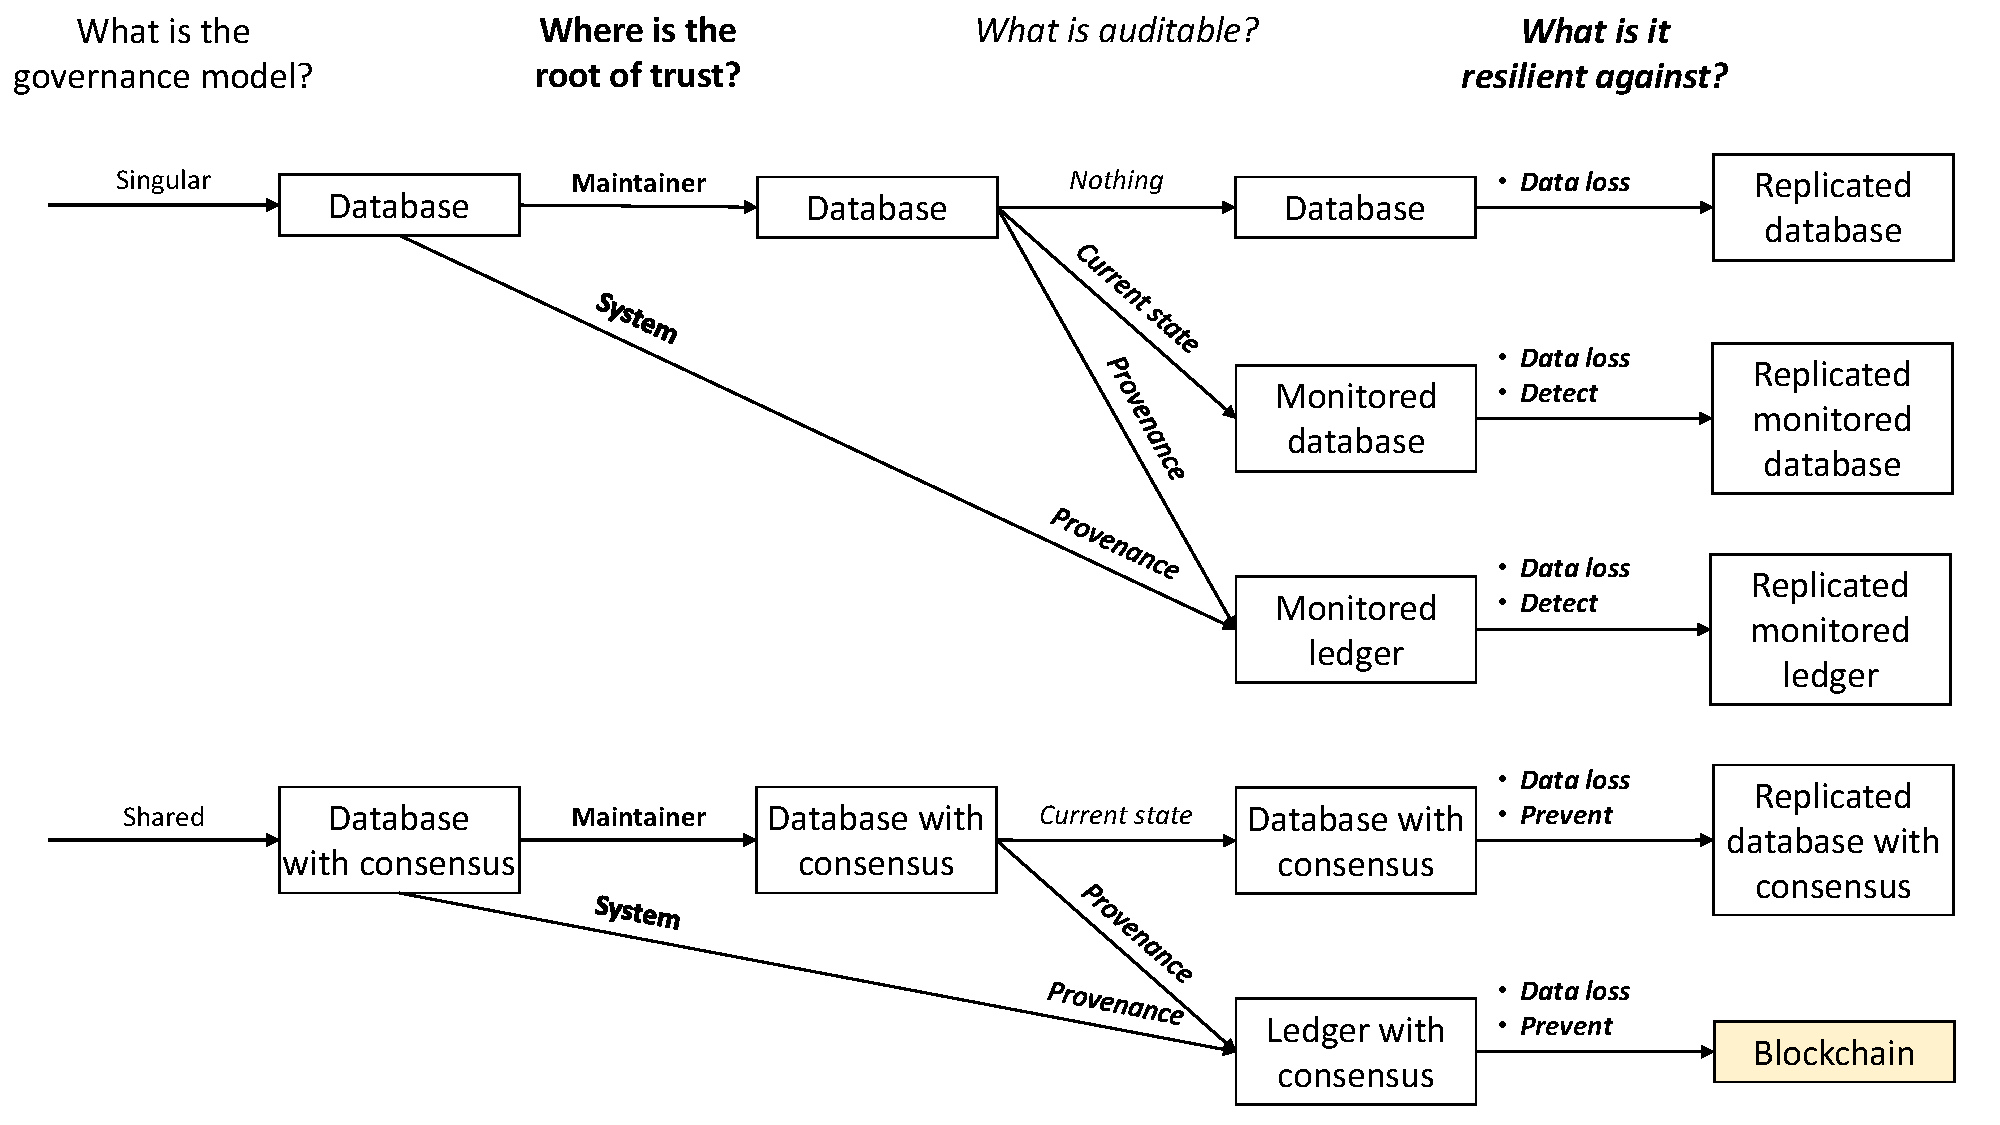
\includegraphics[width=\textwidth]{figures/BlockchainFlowchart}
	\caption{Comparing decentralized databases. Blockchain is highlighted in the bottom right corner.}
	\label{fig:blockchainFlowchart}
\end{figure*}

The first property in our taxonomy considers who has the authority to manage and update the database: \emph{what is the governance model?} In a centrally governed database (``Centralized''), a single entity performs these tasks. Alternatively, the system can use a consensus protocol to allow for decentralized governance (``Decentralized'').

Next, we consider the security model by asking \emph{where is the root of trust?}
This refers to the entity or entities that must behave honestly in order for the system to be secure.
In typical database systems, trust is rooted in the maintainer (``Maintainer'')---for example, using AWS cloud storage requires that you trust Amazon.
Alternatively, trust can be rooted in the design of the system itself (``System''), though this is only possible if the system stores sufficient provenance for it to be audited to confirm that the system is functioning as intended.

The next question is \emph{what is auditable?}
In the worst case, nothing is auditable (``Nothing'').
Systems can use an authenticated data structure~\cite{tamassia2003authenticated} to ensure that their current state can be audited (``Current state'').
If the state also contains a history of the system (e.g., a ledger), then the use of an authenticated data structure allows for the provenance of the system to also be audited (``Provenance'').
In both cases, it is necessary that these databases be monitored to ensure that they never enter an invalid state, even temporarily.
In the case of decentralized systems, the decentralized partners can act as monitors.

Finally, we can classify systems by asking \emph{what is it resilient against?}
In particular, we considered with three resiliency properties---(1) is it resilient to accidental data loss (``Data loss''), (2) is it possible to detect that data has been malicious altered (``Detect''), (3) and is it possible to prevent malicious updates (``Prevent'').
Systems with centralized governance are only able to detect malicious updates as the monitors can detect the attack but cannot prevent the malicious update from being replicated.
If we modify the system to allow monitors to play this role, they have become consensus partners and we now have a decentralized database.

\subsection{Is Blockchain a Good Fit for My Project?}
In Figure~\ref{fig:blockchainFlowchart}, systems increase in complexity and overhead as they move down or to the right.
As such, it is usually preferable to select the first system in the flowchart that meets all of the desired properties.
While Blockchain provides the most functionality, it is also the most complex of the related systems.
As such, while it can be used in place of simpler systems (e.g., a replicated database), we recommend Blockchain technology only be used if the application has most of the following needs:

\begin{enumerate}
	\item It requires shared governance and operation.
	\item It is necessary or desirable to store provenance for the system or the resources managed or controlled by the system.
	\item It requires that the system be audited, particularly if there is a desire to trust the system itself and not the system's maintainer(s).
	\item Replication is necessary to prevent data loss and malicious updates.
\end{enumerate}

\subsection{Normative and Technical Properties are Cleanly Separable}
When reading documents from industry, normative and technical properties are often intermingled with each other.
The injection of ideology into a technical field causes confusion and suboptimal design choices, not to mention muddying discussion and preventing clarity.
In our concept graph, however, technical properties and normative properties cleanly separate.
No capabilities have dependencies on normative properties, and removing them from the graph does not lessen the value of the graph as an exploration of technical concepts.
The fact that this separation occurred naturally indicates that grounded theory accomplished our research goals and was a good choice for addressing this corpus of data.

In general, the normative properties dealt with idealogical-driven goals that could accomplished using Blockchain technology.
For example, several normative properties dealt with public participation, community ownership, censorship resistance, and transparency of Blockchain systems.
Bitcoin demonstrates that Blockchain technology can be used to achieve these properties, but it is not the case that all Blockchain systems will accomplish these goals---for example, Ripple is a Blockchain system without public participation.

\subsection{Lack of Privacy and Data Discoverability}
In the literature we found a common misconception that Blockchain technology inherently provided confidentiality for information stored within it.
In fact the opposite is true, all transactions are visible to all miners and this is necessary for miners to validate transactions.
The global visibility was identified by some as a capability (i.e., data discoverability) that allowed a Blockchain to act as a data lake.
While there were some valid applications of Blockchain as a data lake, in most cases we found that proposed data lake applications did not need all of Blockchain technology's capabilities and that a simpler solution would have sufficed.

It may be possible to add confidentiality to Blockchain technology, but care must be taken to ensure that this confidentiality does not preclude miners ability to validate and audit the system.
This remains an open research problem.

\subsection{Private Governance}
In our survey of the industrial literature, we encountered several systems that claimed to be Blockchain systems, but which did not have shared governance.
These systems resembled Blockchain systems, but with one critical difference: all the miners were controlled by a single entity.
The most prominent example of a private governance system is IBM's HyperLedger Fabric.
Interestingly, the HyperLedger Fabric software project allows for consortium governance, but IBM's implementation has IBM manage all of the miners.

Ultimately, we do not classify such systems as Blockchain technology.
First, these systems do not have shared governance, which we identify as the key component of Blockchain technology.
Second, the party governing the system still represents a single-point of failure.
While the miners within the operating organization might be run on a distributed infrastructure, there is still a high chance that a sufficient compromise in the operating organization would lead to a compromise in the Blockchain system.
Third, there is nothing that prevents the governing party from deleting or modifying data; even if such changes could be detected, the data itself is not replicated outside the organization and would be lost.
Finally, most of the private governance systems are overly complex for what they are trying to accomplish.
Without the need for shared governance, many of these systems could be better implemented as a replicated monitored database.

\subsection{Ideology, Hype, and Ulterior Motives}
Many proponents of Blockchain technology believe that it has the capability to massively disrupt how society operates, or at least to rapidly overtake legacy solutions in many significant industries. This belief is hyperbole (i.e., hype) as though Blockchain technology has many valid uses, it has not, nor is it likely to achieve this Utopian vision. This ideology and hype cause problems: for example, frequent emotionally-charged schisms within Blockchain advocate and developer communities---especially those affiliated with Bitcoin. This turmoil prevents level-headed scientific discourse and wastes developer resources. It can also tangibly affect the stability of a Blockchain systems by causing a fork, in which two independent chains emerge to used and maintained by different groups, further dividing resources.

With that said, Blockchain technology's disruptive power has certainly been demonstrated in the financial sector, so it clearly has promise. Several factors have made this sector an attractive target for disruption, perhaps none more so than the opportunity for massive profit. This motive has had benefits for Blockchain technology, especially in accelerating the pace of technological development. However, it has also created perverse incentives to reinforce hype and ideology. Hype can attract investors and inflate valuations, and dogmatic ideology is a proven marketing and recruitment strategy for financial scammers. These problems inhibit the advancement of Blockchain technology.

\subsection{Reputation for illicit uses}
Due to the prominence of Bitcoin, many people are familiar with Blockchain first and foremost as the technology underlying the cryptocurrency and therefore the reputations of the two are intertwined. The fact that Bitcoin is designed to avoid banks and central authorities in general, combined with its well-known history of illicit uses, somewhat poisons the well for Blockchain as a whole. Along with the causes listed above (ideology, hype, and ulterior motives), this contributes to the difficulty of discussing and considering Blockchain technology with precision and objectivity. It may also have impeded or delayed its acceptance by organizations unwilling to associate themselves with the technology's poor reputation.

%\subsubsection{Anonymity is Orthogonal to Blockchain Technology}
%Several sources in our dataset refer to anonymity as a key feature of Blockchain technology.
%While it is true that Blockchain systems can allow for anonymous transactions, an analysis of our result graph shows that anonymity is only weakly connected to the rest of the group.
%Thus, while anonymity is often discussed as one of the exciting properties related to Blockchain technology, it doesn't a

\snote{Discuss side chains and layer 2 approaches.}